% ============================================================
%  Chapter: The MyPath Routing Engine
%  Description: A full technical chapter on the MyPath
%  wheelchair-accessible routing backend.
% ============================================================

\documentclass[12pt, a4paper]{report}

% ---------- Packages ----------
\usepackage[utf8]{inputenc}
\usepackage[T1]{fontenc}
\usepackage{lmodern}
\usepackage[margin=1in]{geometry}
\usepackage{graphicx}
\usepackage{xcolor}
\usepackage{hyperref}
\usepackage{booktabs}
\usepackage{tabularx}
\usepackage{array}
\usepackage{enumitem}
\usepackage{tcolorbox}
\usepackage{tikz}
\usepackage{pgf-umlsd}
\usepackage{float}
\usepackage{amsmath}
\usepackage{microtype}
\usepackage{fancyhdr}
\usepackage{titlesec}
\usepackage{parskip}
\usepackage{caption}
\usepackage{mdframed}
\usepackage{multirow}
\usepackage{longtable}

\usetikzlibrary{shapes.geometric, arrows.meta, positioning, fit, backgrounds, shadows}

% ---------- Colours ----------
\definecolor{myblue}{HTML}{0ea5e9}
\definecolor{mypurple}{HTML}{8b5cf6}
\definecolor{mygreen}{HTML}{10b981}
\definecolor{myorange}{HTML}{f97316}
\definecolor{myred}{HTML}{ef4444}
\definecolor{myyellow}{HTML}{eab308}
\definecolor{myindigo}{HTML}{6366f1}
\definecolor{lightgray}{HTML}{f1f5f9}
\definecolor{darkgray}{HTML}{334155}

% ---------- Hyperlink colours ----------
\hypersetup{
    colorlinks=true,
    linkcolor=myindigo,
    urlcolor=myblue,
    citecolor=mypurple,
}

% ---------- Header / Footer ----------
\pagestyle{fancy}
\fancyhf{}
\fancyhead[L]{\small\textit{MyPath Routing Engine}}
\fancyhead[R]{\small\textit{Technical Documentation}}
\fancyfoot[C]{\thepage}
\renewcommand{\headrulewidth}{0.4pt}

% ---------- Section formatting ----------
\titleformat{\chapter}[display]
  {\normalfont\huge\bfseries\color{darkgray}}
  {\chaptertitlename\ \thechapter}{18pt}{\Huge}

\titleformat{\section}{\large\bfseries\color{myindigo}}{}{0em}{\thesection\quad}
\titleformat{\subsection}{\normalsize\bfseries\color{myblue}}{}{0em}{\thesubsection\quad}
\titleformat{\subsubsection}{\normalsize\bfseries\color{mypurple}}{}{0em}{\thesubsubsection\quad}

% ---------- TColorBox styles ----------
\tcbuselibrary{skins, breakable, listings}

\newtcolorbox{infobox}[1][]{
  colback=myblue!8, colframe=myblue, arc=6pt,
  fonttitle=\bfseries\small, title={#1},
  boxrule=1.2pt, left=8pt, right=8pt, top=6pt, bottom=6pt
}

\newtcolorbox{warningbox}[1][]{
  colback=myorange!8, colframe=myorange, arc=6pt,
  fonttitle=\bfseries\small, title={#1},
  boxrule=1.2pt, left=8pt, right=8pt, top=6pt, bottom=6pt
}

\newtcolorbox{keybox}[1][]{
  colback=mypurple!8, colframe=mypurple, arc=6pt,
  fonttitle=\bfseries\small, title={#1},
  boxrule=1.2pt, left=8pt, right=8pt, top=6pt, bottom=6pt
}

\newtcolorbox{greenbox}[1][]{
  colback=mygreen!8, colframe=mygreen, arc=6pt,
  fonttitle=\bfseries\small, title={#1},
  boxrule=1.2pt, left=8pt, right=8pt, top=6pt, bottom=6pt
}

% ============================================================
\begin{document}

\tableofcontents
\newpage

% ============================================================
\chapter{The MyPath Routing Engine}
\label{chap:mypath}

% ============================================================
\section{Introduction and Motivation}
\label{sec:intro}

Navigation technology has transformed how people move through the world. Yet for the more than 70 million wheelchair users worldwide, mainstream routing engines — designed around the assumptions of pedestrians who can climb steps, traverse gravel paths, or manage steep inclines — consistently produce routes that are physically inaccessible or dangerous. MyPath is a specialised backend routing engine built to close this gap.

MyPath generates wheelchair-accessible navigation routes by combining three mature technologies: the \textbf{GraphHopper} open-source routing engine, \textbf{OpenStreetMap (OSM)} geographic data, and \textbf{SRTM} three-dimensional elevation data. Together they enable MyPath to reason not only about which roads and paths exist on a map, but about the physical properties of those paths — their surface material, gradient, smoothness, and road classification — and to select routes that a wheelchair user can actually traverse safely and comfortably.

The engine exposes a clean HTTP REST interface and is designed to operate continuously, updating its internal map data every day without restarting the server. This chapter provides a comprehensive technical description of every aspect of the system: its architecture, data model, routing logic, navigation processing, security design, and operational lifecycle.

% ============================================================
\section{System Architecture Overview}
\label{sec:architecture}

At the highest level, MyPath is a Spring Boot application running on port 8093. It acts as an intelligent middleware layer between a client application (typically a web or mobile frontend) and the underlying graph-based routing engine. Figure~\ref{fig:architecture} illustrates the principal architectural layers.

\begin{figure}[H]
\centering
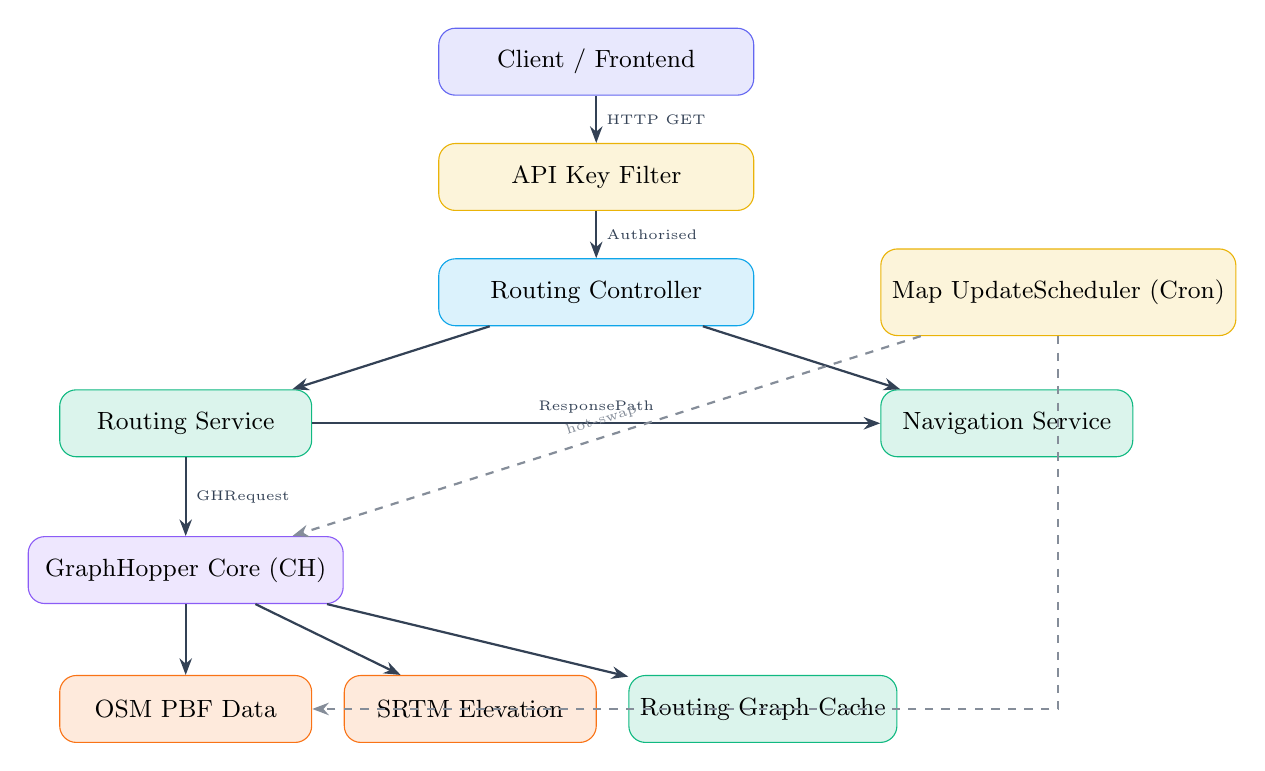
\begin{tikzpicture}[
  node distance=0.6cm and 1.2cm,
  box/.style={rectangle, rounded corners=6pt, draw, minimum width=3.2cm, minimum height=0.85cm, text centered, font=\small, inner sep=4pt},
  bluebox/.style={box, fill=myblue!15, draw=myblue},
  greenbox_s/.style={box, fill=mygreen!15, draw=mygreen},
  purplebox/.style={box, fill=mypurple!15, draw=mypurple},
  orangebox/.style={box, fill=myorange!15, draw=myorange},
  yellowbox/.style={box, fill=myyellow!15, draw=myyellow},
  indigobox/.style={box, fill=myindigo!15, draw=myindigo},
  redbox/.style={box, fill=myred!15, draw=myred},
  arr/.style={-{Stealth[length=6pt]}, thick, color=darkgray},
  dasharr/.style={-{Stealth[length=6pt]}, thick, dashed, color=darkgray!60},
]

%% Client
\node[indigobox, minimum width=4cm] (client) {Client / Frontend};

%% Filter
\node[yellowbox, below=of client, minimum width=4cm] (filter) {API Key Filter};

%% Controller
\node[bluebox, below=of filter, minimum width=4cm] (ctrl) {Routing Controller};

%% Services
\node[greenbox_s, below left=0.8cm and 1.6cm of ctrl] (routing) {Routing Service};
\node[greenbox_s, below right=0.8cm and 1.6cm of ctrl] (nav) {Navigation Service};

%% GraphHopper
\node[purplebox, below=1.0cm of routing, minimum width=4cm] (gh) {GraphHopper Core (CH)};

%% Data layer
\node[orangebox, below=0.9cm of gh] (osm) {OSM PBF Data};
\node[orangebox, right=0.4cm of osm] (srtm) {SRTM Elevation};
\node[greenbox_s, right=0.4cm of srtm] (cache) {Routing Graph Cache};

%% Cron
\node[yellowbox, right=1.6cm of ctrl, minimum width=3cm, minimum height=1.1cm] (cron) {Map Update\\Scheduler (Cron)};

%% Arrows
\draw[arr] (client) -- (filter) node[midway, right, font=\tiny] {HTTP GET};
\draw[arr] (filter) -- (ctrl) node[midway, right, font=\tiny] {Authorised};
\draw[arr] (ctrl) -- (routing);
\draw[arr] (ctrl) -- (nav);
\draw[arr] (routing) -- (gh) node[midway, right, font=\tiny] {GHRequest};
\draw[arr] (gh) -- (osm);
\draw[arr] (gh) -- (srtm);
\draw[arr] (gh) -- (cache);
\draw[arr] (routing) -- (nav) node[midway, above, font=\tiny] {ResponsePath};
\draw[dasharr] (cron) -- (gh) node[midway, above, font=\tiny, sloped] {hot-swap};
\draw[dasharr] (cron) |- (osm);

\end{tikzpicture}
\caption{High-level system architecture of the MyPath routing engine.}
\label{fig:architecture}
\end{figure}

The system can be divided into four conceptual tiers:

\begin{enumerate}[leftmargin=*, label=\textbf{\arabic*.}]
  \item \textbf{Security Tier.} Every incoming HTTP request passes through the \texttt{ApiKeyFilter} before reaching any business logic. Requests without a valid Bearer token are rejected immediately with an HTTP 401 response.
  \item \textbf{Service Tier.} The \texttt{RoutingService} translates client coordinates into a GraphHopper query, while the \texttt{NavigationService} transforms the raw graph response into a structured, client-friendly representation.
  \item \textbf{Routing Engine Tier.} GraphHopper provides the computational core: it stores a preprocessed road network graph, applies the wheelchair-specific routing profile, and returns an optimal path.
  \item \textbf{Data Tier.} Raw geographic data comes from OpenStreetMap PBF files. Elevation comes from NASA's SRTM dataset. A preprocessed routing graph cache accelerates query time dramatically.
\end{enumerate}

% ============================================================
\section{Technology Stack}
\label{sec:stack}

Table~\ref{tab:stack} lists the primary components, their versions, and the roles they play within MyPath.

\begin{table}[H]
\centering
\caption{MyPath technology stack}
\label{tab:stack}
\begin{tabularx}{\textwidth}{@{}lllX@{}}
\toprule
\textbf{Component} & \textbf{Version} & \textbf{Role} \\
\midrule
Spring Boot & 3.4.3 & Application framework, REST API, dependency injection, scheduling \\
GraphHopper Core & 10.2 & Graph-based routing engine with CH optimisation \\
Osmosis Core + PBF & 0.49.2 & OSM PBF file reading and processing \\
SRTM Provider & — & 3D terrain elevation data integration \\
Java SDK & 17+ & Runtime environment \\
Gradle & 8.7 & Build automation \\
SLF4J + Logback & 2.0 / 1.5 & Structured application logging \\
\bottomrule
\end{tabularx}
\end{table}

% ============================================================
\section{Geographic Data Sources}
\label{sec:datasources}

A routing engine's accuracy is only as good as the data it reasons over. MyPath draws from two independently maintained, high-quality geographic datasets.

\subsection{OpenStreetMap PBF Files}
\label{subsec:osm}

OpenStreetMap (OSM) is a collaboratively edited, freely available world map. MyPath consumes OSM data in the Protocol Buffer Binary (PBF) format — a compact, efficient binary encoding of the XML-based OSM data model. PBF files are downloaded from \textbf{Geofabrik}, a service that publishes daily regional extracts of the OSM planet.

Each PBF file encodes the road and path network as a graph of \emph{nodes} (geographic points with latitude and longitude), \emph{ways} (ordered sequences of nodes forming roads, paths, or areas), and \emph{relations} (logical groupings of nodes and ways). Every way carries \emph{tags} — key-value pairs that describe physical properties including surface type, road classification, smoothness, footway designation, and access restrictions.

MyPath supports the following regional extracts out of the box:

\begin{table}[H]
\centering
\caption{Supported OSM PBF regional extracts}
\begin{tabular}{@{}ll@{}}
\toprule
\textbf{Region} & \textbf{Source} \\
\midrule
Maryland & \texttt{maryland-latest.osm.pbf} via Geofabrik \\
Ohio & \texttt{ohio-latest.osm.pbf} via Geofabrik \\
Wisconsin & \texttt{wisconsin-latest.osm.pbf} via Geofabrik \\
United States (full) & \texttt{us-latest.osm.pbf} via Geofabrik \\
\bottomrule
\end{tabular}
\end{table}

Smaller regional extracts are preferred for deployments serving a specific area because they dramatically reduce startup time and memory footprint compared to a full-country extract.

\subsection{SRTM Elevation Data}
\label{subsec:srtm}

The Shuttle Radar Topography Mission (SRTM) is a NASA programme that produced near-global terrain elevation data at approximately 30-metre resolution. MyPath integrates the \texttt{SRTMProvider} supplied with GraphHopper, which enriches every coordinate in the routing graph with a third dimension: altitude above sea level.

This elevation data serves two critical purposes. First, it allows the routing profile to impose speed and priority penalties based on terrain steepness, protecting users from being routed onto gradients that a manual wheelchair cannot safely manage. Second, it allows per-segment incline percentages to be reported in the API response, giving the client application the information needed to provide appropriate warnings or to render elevation profiles.

% ============================================================
\section{The GraphHopper Routing Engine}
\label{sec:graphhopper}

GraphHopper is the computational heart of MyPath. It is an open-source, Java-based routing engine that transforms the raw OSM graph data into a highly optimised in-memory routing structure.

\subsection{Graph Representation}
\label{subsec:graph}

When MyPath first starts (or after a daily map update), GraphHopper reads the PBF file and constructs an internal directed graph. Each navigable segment of road or path becomes an \emph{edge} in this graph; each junction or endpoint becomes a \emph{node}. The graph is then enriched with \emph{encoded values} — a compact numerical representation of the OSM tags relevant to the wheelchair profile.

MyPath configures GraphHopper to index the following encoded values:

\begin{center}
\begin{tikzpicture}
  \foreach \label/\col [count=\i] in {
    foot\_access/myblue,
    hike\_rating/myblue,
    mtb\_rating/myblue,
    foot\_priority/mygreen,
    foot\_average\_speed/mygreen,
    average\_slope/myred,
    max\_slope/myred,
    surface/mypurple,
    footway/mypurple,
    smoothness/mypurple,
    country/darkgray,
    road\_class/darkgray
  } {
    \pgfmathsetmacro{\row}{int((\i-1)/4)}
    \pgfmathsetmacro{\col_idx}{int(mod(\i-1,4))}
    \node[rectangle, rounded corners=4pt, fill=\col!15, draw=\col, font=\tiny\ttfamily,
          minimum width=2.4cm, minimum height=0.5cm, text centered]
      at (\col_idx * 2.7, -\row * 0.75) {\label};
  }
\end{tikzpicture}
\end{center}

These encoded values are stored efficiently in the graph and are available to the routing profile at query time without any additional database lookups.

\subsection{Contraction Hierarchies}
\label{subsec:ch}

Routing on a graph the size of a regional or national road network is computationally expensive. A naive Dijkstra search would need to evaluate millions of edges. MyPath addresses this through \textbf{Contraction Hierarchies (CH)}, a well-established graph preprocessing technique.

During graph construction (at startup or after a map update), GraphHopper computes a hierarchy of ``shortcuts'' across the graph. Low-importance nodes are \emph{contracted} out of the graph, and shortcut edges are added to preserve path optimality without requiring evaluation of every intermediate node. The result is a layered graph structure in which high-level routes can be resolved in milliseconds even over large geographic regions.

The CH preprocessing is stored in the routing graph cache directory (\texttt{myPathDataStore/routing-graph-cache/}) so that subsequent server restarts do not need to repeat the expensive computation — only importing or loading the pre-built cache.

\begin{infobox}[Why CH Matters for Accessibility Routing]
Standard routing profiles treat all road types as potential candidates and simply apply weights. An accessibility-aware profile must hard-exclude many road types while also applying continuous gradient penalties. The CH algorithm handles this correctly: it optimises over the modified, penalised graph, not over the raw network. Queries that return in under 10 milliseconds are typical even on full-state extracts.
\end{infobox}

\subsection{Graph Cache Lifecycle}
\label{subsec:cache}

The routing graph cache is a serialised form of the preprocessed CH graph stored to disk. MyPath uses two cache paths:

\begin{itemize}[leftmargin=*]
  \item \textbf{Primary cache} (\texttt{routing-graph-cache/}): the cache currently in active use by the live server.
  \item \textbf{Temporary cache} (\texttt{routing-graph-cache-tmp/}): built from a fresh PBF file during a daily update, before being atomically promoted to the primary slot.
\end{itemize}

The use of a temporary cache ensures that the server never operates on a partially-built graph.

% ============================================================
\section{The Wheelchair Custom Routing Profile}
\label{sec:profile}

The most critical distinction between MyPath and a generic routing engine is its wheelchair-specific routing profile. The profile is defined in a JSON file (\texttt{wheelchair.json}) and consumed by GraphHopper as a \emph{custom model}. It governs two independent dimensions of routing quality: \textbf{priority} (which paths to prefer or avoid) and \textbf{speed} (how fast travel on a segment is modelled).

\subsection{Priority Rules}
\label{subsec:priority}

Priority rules multiply a base priority score to make certain paths more or less attractive. A multiplier of zero means the path is completely forbidden; a multiplier of one means full priority. Figure~\ref{fig:priority} illustrates the decision logic.

\begin{figure}[H]
\centering
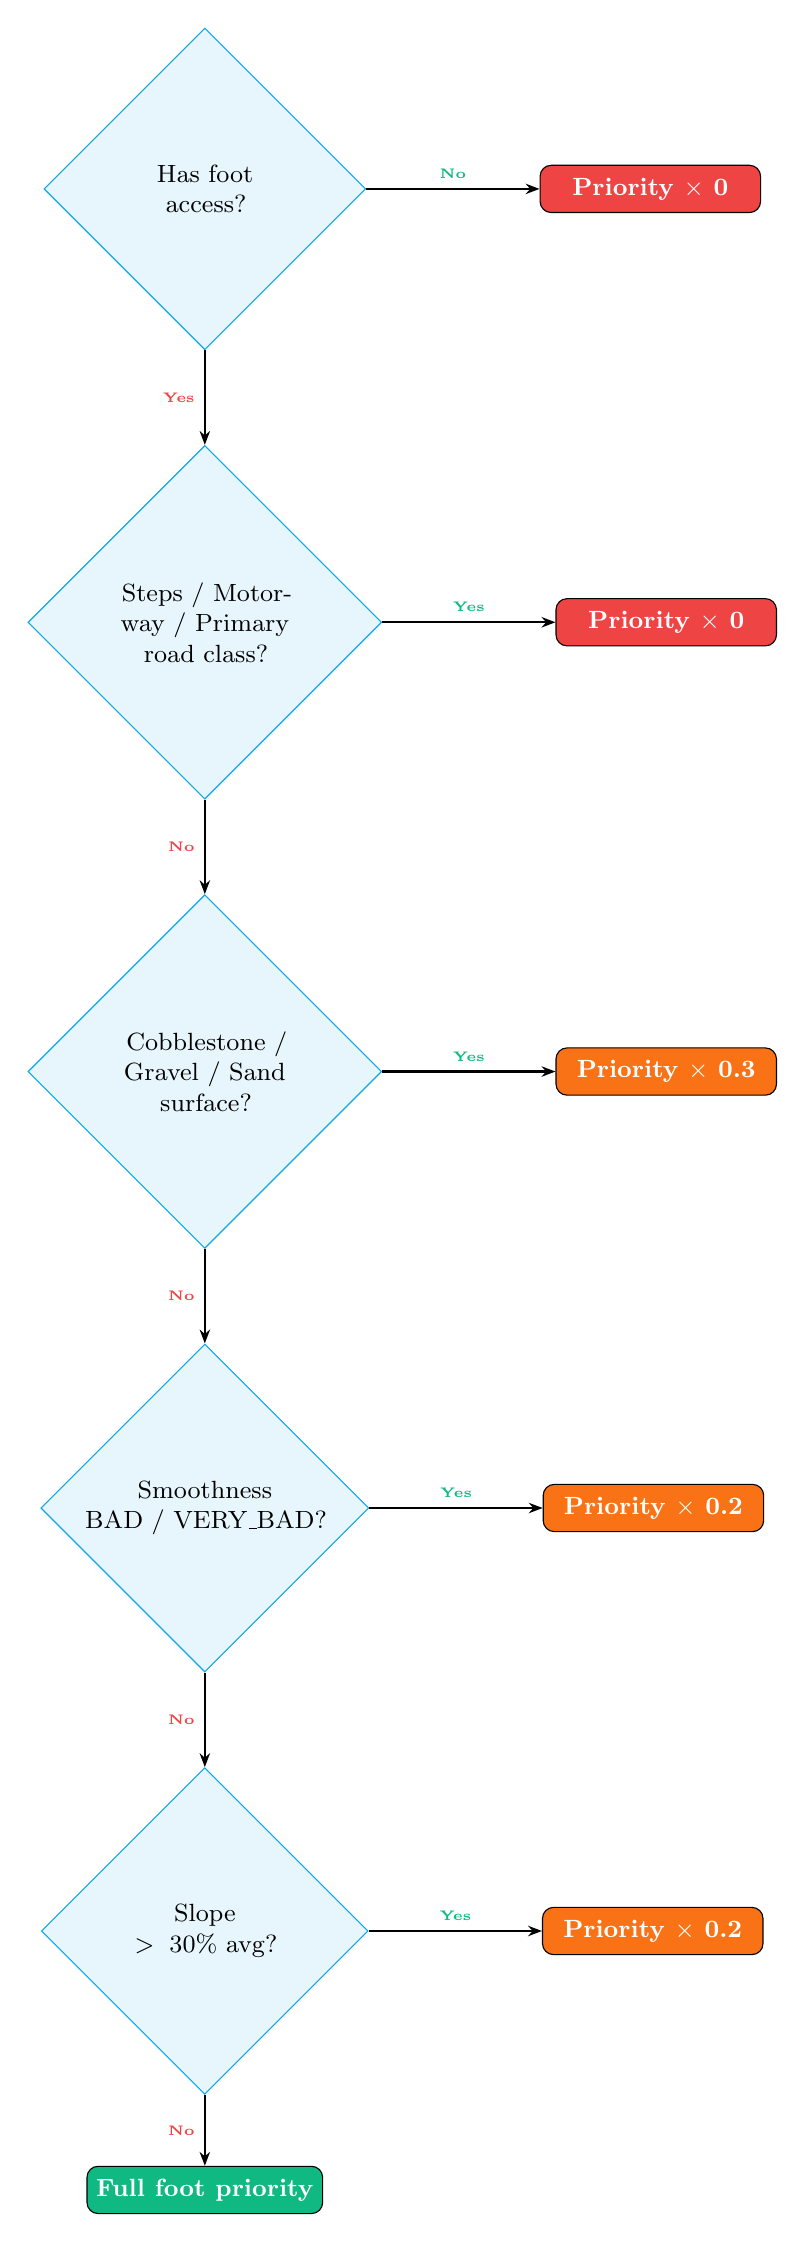
\begin{tikzpicture}[
  decision/.style={diamond, draw=myblue, fill=myblue!10, text width=3.2cm, align=center, font=\small, inner sep=2pt},
  result/.style={rectangle, rounded corners=4pt, draw, fill, text=white, font=\small\bfseries, minimum width=2.8cm, minimum height=0.6cm, text centered},
  arr/.style={-{Stealth[length=5pt]}, thick},
  yes/.style={font=\tiny\bfseries, color=mygreen},
  no/.style={font=\tiny\bfseries, color=myred},
]
\node[decision] (d1) {Has foot\\access?};
\node[result, fill=myred, right=2.2cm of d1] (r0a) {Priority $\times$ 0};
\node[decision, below=1.2cm of d1] (d2) {Steps / Motor-\\way / Primary\\road class?};
\node[result, fill=myred, right=2.2cm of d2] (r0b) {Priority $\times$ 0};
\node[decision, below=1.2cm of d2] (d3) {Cobblestone /\\Gravel / Sand\\surface?};
\node[result, fill=myorange, right=2.2cm of d3] (r03) {Priority $\times$ 0.3};
\node[decision, below=1.2cm of d3] (d4) {Smoothness\\BAD / VERY\_BAD?};
\node[result, fill=myorange, right=2.2cm of d4] (r02) {Priority $\times$ 0.2};
\node[decision, below=1.2cm of d4] (d5) {Slope\\ $> 30\%$ avg?};
\node[result, fill=myorange, right=2.2cm of d5] (r02b) {Priority $\times$ 0.2};
\node[result, fill=mygreen, below=0.9cm of d5] (rOK) {Full foot priority};

\draw[arr] (d1) -- node[yes, above] {No} (r0a);
\draw[arr] (d1) -- node[no, left] {Yes} (d2);
\draw[arr] (d2) -- node[yes, above] {Yes} (r0b);
\draw[arr] (d2) -- node[no, left] {No} (d3);
\draw[arr] (d3) -- node[yes, above] {Yes} (r03);
\draw[arr] (d3) -- node[no, left] {No} (d4);
\draw[arr] (d4) -- node[yes, above] {Yes} (r02);
\draw[arr] (d4) -- node[no, left] {No} (d5);
\draw[arr] (d5) -- node[yes, above] {Yes} (r02b);
\draw[arr] (d5) -- node[no, left] {No} (rOK);
\end{tikzpicture}
\caption{Wheelchair profile priority decision tree. Penalties are multiplicative and cascade.}
\label{fig:priority}
\end{figure}

The full set of priority rules is summarised in Table~\ref{tab:priority}.

\begin{table}[H]
\centering
\caption{Wheelchair profile priority rules}
\label{tab:priority}
\begin{tabularx}{\textwidth}{@{}lXl@{}}
\toprule
\textbf{Condition} & \textbf{Rationale} & \textbf{Multiplier} \\
\midrule
No foot access & Path is legally or physically off-limits & $\times 0$ \\
Steps / Motorways / Primary roads & Impassable or unsafe for wheelchairs & $\times 0$ \\
Cobblestone, gravel, or sand surface & Highly difficult to traverse & $\times 0.3$ \\
Smoothness rated BAD or VERY\_BAD & Pavement too rough for safe use & $\times 0.2$ \\
Max slope exceeds 50\% & Dangerously steep & $\times 0$ \\
Average slope exceeds 30\% & Extremely steep, generally impassable & $\times 0.2$ \\
Average slope exceeds 20\% & Very steep; strongly discouraged & $\times 0.5$ \\
All other accessible footways & Normal traversal & $\times 1.0$ \\
\bottomrule
\end{tabularx}
\end{table}

\subsection{Speed Rules}
\label{subsec:speed}

Speed rules place an upper bound on the modelled travel speed for a segment. They do not affect which path is chosen (that is the priority's job) but they affect the estimated duration of travel, which is surfaced in the API response and can influence the CH graph's cost function.

\begin{table}[H]
\centering
\caption{Wheelchair profile speed caps by terrain condition}
\begin{tabular}{@{}ll@{}}
\toprule
\textbf{Condition} & \textbf{Speed Cap} \\
\midrule
Max slope $> 50\%$ & 3 km/h \\
Max slope $> 10\%$ & 2 km/h \\
Average slope $> 30\%$ & 4 km/h \\
Average slope $> 20\%$ & 5 km/h \\
Normal accessible path & \texttt{foot\_average\_speed} (OSM tag) \\
\bottomrule
\end{tabular}
\end{table}

% ============================================================
\section{API Design and Security}
\label{sec:api}

\subsection{Endpoint Structure}
\label{subsec:endpoint}

MyPath exposes a single primary routing endpoint:

\begin{center}
\texttt{GET http://\textit{host}:8093/route/getSingleRoute}
\end{center}

The endpoint accepts four query parameters:

\begin{table}[H]
\centering
\caption{Query parameters for the routing endpoint}
\begin{tabular}{@{}llll@{}}
\toprule
\textbf{Parameter} & \textbf{Type} & \textbf{Description} \\
\midrule
\texttt{srcLat} & \texttt{double} & Source latitude (decimal degrees) \\
\texttt{srcLon} & \texttt{double} & Source longitude (decimal degrees) \\
\texttt{destLat} & \texttt{double} & Destination latitude (decimal degrees) \\
\texttt{destLon} & \texttt{double} & Destination longitude (decimal degrees) \\
\bottomrule
\end{tabular}
\end{table}

\subsection{Bearer Token Authentication}
\label{subsec:auth}

All requests to the \texttt{/route/*} path family must include an \texttt{Authorization} header carrying a pre-shared Bearer token:

\begin{center}
\texttt{Authorization: Bearer \textit{<api-key>}}
\end{center}

The \texttt{ApiKeyFilter} intercepts every request before it reaches the controller. It extracts the token from the header and compares it against the value configured in \texttt{application.properties}. If the comparison fails or the header is absent, the filter immediately terminates the request with an HTTP \texttt{401 Unauthorized} response, preventing any routing computation from occurring.

This design follows the \emph{fail-fast} security principle: unauthenticated requests never exercise any server-side logic beyond the filter itself.

\subsection{Error Responses}
\label{subsec:errors}

\begin{table}[H]
\centering
\caption{API error response codes}
\begin{tabular}{@{}cll@{}}
\toprule
\textbf{HTTP Status} & \textbf{Condition} & \textbf{Handler} \\
\midrule
401 & Missing or invalid Authorization header & \texttt{ApiKeyFilter} \\
404 & No accessible wheelchair route found & \texttt{GlobalExceptionHandler} \\
\bottomrule
\end{tabular}
\end{table}

The \texttt{GlobalExceptionHandler} catches the custom \texttt{RouteNotFound} exception thrown by the navigation pipeline and translates it into a standard HTTP 404 response with a descriptive message body.

% ============================================================
\section{The Route Processing Pipeline}
\label{sec:pipeline}

Once a request clears authentication and reaches the service layer, it passes through a multi-stage processing pipeline before a response is returned. This pipeline is illustrated in Figure~\ref{fig:pipeline} and described in detail in the subsections below.

\begin{figure}[H]
\centering
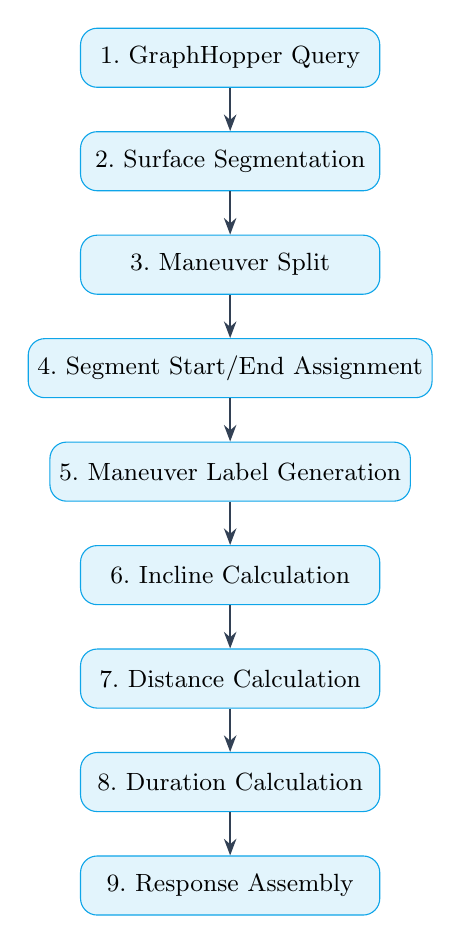
\begin{tikzpicture}[
  stage/.style={rectangle, rounded corners=6pt, draw=myblue, fill=myblue!12, minimum width=3.8cm, minimum height=0.75cm, font=\small, text centered},
  arr/.style={-{Stealth[length=6pt]}, thick, color=darkgray},
  node distance=0.55cm,
]
\node[stage] (s1) {1.\ GraphHopper Query};
\node[stage, below=of s1] (s2) {2.\ Surface Segmentation};
\node[stage, below=of s2] (s3) {3.\ Maneuver Split};
\node[stage, below=of s3] (s4) {4.\ Segment Start/End Assignment};
\node[stage, below=of s4] (s5) {5.\ Maneuver Label Generation};
\node[stage, below=of s5] (s6) {6.\ Incline Calculation};
\node[stage, below=of s6] (s7) {7.\ Distance Calculation};
\node[stage, below=of s7] (s8) {8.\ Duration Calculation};
\node[stage, below=of s8] (s9) {9.\ Response Assembly};

\draw[arr] (s1) -- (s2);
\draw[arr] (s2) -- (s3);
\draw[arr] (s3) -- (s4);
\draw[arr] (s4) -- (s5);
\draw[arr] (s5) -- (s6);
\draw[arr] (s6) -- (s7);
\draw[arr] (s7) -- (s8);
\draw[arr] (s8) -- (s9);
\end{tikzpicture}
\caption{The nine-stage route processing pipeline in \texttt{NavigationService}.}
\label{fig:pipeline}
\end{figure}

\subsection{Stage 1: GraphHopper Query}
\label{subsec:stage1}

The \texttt{RoutingService} constructs a \texttt{GHRequest} object with the source and destination coordinates, specifies the \texttt{wheelchair} profile, and requests three path detail layers: \texttt{surface}, \texttt{street\_name}, and \texttt{footway}. Path details are GraphHopper's mechanism for attaching attribute metadata (from the encoded value graph) to contiguous ranges of the returned path's point list.

The \texttt{GraphHopper} instance executes the query against the CH-preprocessed graph and returns a \texttt{GHResponse}. If GraphHopper reports errors or returns no response, a \texttt{RouteNotFound} exception is thrown immediately.

\subsection{Stage 2: Surface Segmentation}
\label{subsec:stage2}

The raw GraphHopper response contains the full ordered list of 3D coordinates forming the route, together with a surface path detail list. Each entry in the surface list describes a contiguous range of coordinates sharing the same surface type. The navigation service iterates over these ranges, creating one \texttt{Point} segment object per range. Each segment carries the surface type (\textit{asphalt}, \textit{gravel}, \textit{grass}, etc.) and its slice of the coordinate array.

This segmentation is fundamental to the user experience: a client application can render each segment in a different colour on a map, immediately conveying where a path changes from smooth asphalt to rough gravel.

\subsection{Stage 3: Maneuver-Based Splitting}
\label{subsec:stage3}

The surface segmentation produces segments that may contain internal direction changes. Stage 3 walks through every segment's coordinate list and detects turns by computing the \emph{heading change} between consecutive coordinate triplets using the bearing formula described in Section~\ref{sec:geomath}. When a significant direction change is detected within a segment, the segment is split at that point, producing a new segment with the same surface type but representing a distinct leg of travel.

Segments containing only two coordinates (a single straight line) are passed through unchanged.

\subsection{Stage 4: Segment Start and End Assignment}
\label{subsec:stage4}

Once splitting is complete, every segment is assigned its explicit start and end coordinates — the first and last elements of its coordinate list, respectively. These are stored as distinct \texttt{start\_location} and \texttt{end\_location} fields in the \texttt{Point} model, making them directly accessible in the API response without the client needing to inspect the full coordinate list.

\subsection{Stage 5: Maneuver Label Generation}
\label{subsec:stage5}

For each segment (except the final one), the system looks ahead to the next segment to determine the turning instruction the user will need at the end of the current segment. Three coordinates are used: the second-to-last coordinate of the current segment, the last coordinate of the current segment (the junction point), and the second coordinate of the next segment. The heading change between these three points determines which \texttt{TurnDirection} label to assign. The final segment is always labelled \texttt{Reached}.

Table~\ref{tab:maneuver} lists all possible maneuver values.

\begin{table}[H]
\centering
\caption{Maneuver instruction labels and their meanings}
\label{tab:maneuver}
\begin{tabular}{@{}ll@{}}
\toprule
\textbf{Label} & \textbf{Condition} \\
\midrule
Go straight & Heading change $\leq 15°$ \\
Turn slightly left & Heading change between $-15°$ and $-45°$ \\
Turn left & Heading change between $-45°$ and $-135°$ \\
Make a steep left turn & Heading change $< -135°$ \\
Turn slightly right & Heading change between $15°$ and $45°$ \\
Turn right & Heading change between $45°$ and $135°$ \\
Make a steep right turn & Heading change $> 135°$ \\
Reached & Final segment \\
\bottomrule
\end{tabular}
\end{table}

\subsection{Stage 6: Incline Calculation}
\label{subsec:stage6}

For each segment, the incline percentage is computed from the start and end elevation values (derived from SRTM data embedded in the 3D coordinates) and the horizontal distance between start and end. The formula is:

\begin{equation}
  \text{Incline (\%)} = \frac{\Delta h}{d_{\text{horizontal}}} \times 100
\end{equation}

where $\Delta h$ is the elevation change in metres (positive for uphill, negative for downhill) and $d_{\text{horizontal}}$ is the Haversine distance in metres between the start and end coordinates. A positive incline indicates an uphill segment; a negative incline indicates a descent.

\subsection{Stage 7: Distance Calculation}
\label{subsec:stage7}

The per-segment distance is computed by summing the Haversine distances between each consecutive pair of coordinates within the segment. This produces the true path length rather than the straight-line distance between start and end, correctly accounting for curves and bends. The result is expressed both in \textbf{feet} (as a numeric value for calculation) and \textbf{miles} (as a human-readable text string).

\subsection{Stage 8: Duration Calculation}
\label{subsec:stage8}

The estimated travel time for each segment is derived from its distance and a fixed average wheelchair speed constant. The result is expressed in \textbf{seconds} as the primary value, with a \textbf{minutes} text string provided for display. The constant average speed approximates typical manual wheelchair propulsion on level ground; the profile's speed caps ensure that steep segments are already modelled with reduced traversal speed at the GraphHopper level.

\subsection{Stage 9: Response Assembly}
\label{subsec:stage9}

The fully annotated list of \texttt{Point} segments is assembled into a \texttt{Route} object, which is wrapped in a top-level \texttt{Response} object. Spring Boot's built-in JSON serialiser converts this object graph into the final JSON response body returned to the client.

% ============================================================
\section{Geodetic Mathematics}
\label{sec:geomath}

Two fundamental geodetic computations underpin the navigation pipeline: distance calculation using the Haversine formula, and direction determination using forward bearing.

\subsection{The Haversine Formula}
\label{subsec:haversine}

The surface distance between two geographic points — expressed as latitude/longitude pairs — cannot be computed with simple Euclidean geometry because the Earth is spherical. MyPath uses the \emph{Haversine formula}, which gives the great-circle distance between two points on a sphere:

\begin{equation}
  a = \sin^2\!\left(\frac{\Delta\phi}{2}\right) + \cos\phi_1 \cdot \cos\phi_2 \cdot \sin^2\!\left(\frac{\Delta\lambda}{2}\right)
\end{equation}

\begin{equation}
  d = 2R \cdot \arcsin\!\left(\sqrt{a}\right)
\end{equation}

where $\phi$ denotes latitude in radians, $\lambda$ denotes longitude in radians, $\Delta\phi$ and $\Delta\lambda$ are the coordinate differences, and $R = 6{,}371$ km is the mean Earth radius. The result is the shortest surface distance between the two points.

\subsection{Forward Bearing}
\label{subsec:bearing}

The bearing (compass direction) from point $A$ to point $B$ is computed as:

\begin{equation}
  \theta = \arctan2\!\left(\sin(\Delta\lambda)\cdot\cos\phi_B,\;\; \cos\phi_A \cdot \sin\phi_B - \sin\phi_A \cdot \cos\phi_B \cdot \cos(\Delta\lambda)\right)
\end{equation}

The result is normalised to the range $[0°, 360°)$. To detect a turn at point $B$ (given approach from $A$ and departure toward $C$), the heading change is computed as:

\begin{equation}
  \Delta\theta = \left(\theta_{BC} - \theta_{AB} + 360°\right) \bmod 360°
\end{equation}

Values outside $(-180°, +180°)$ are normalised by adding or subtracting $360°$. The magnitude and sign of the resulting heading change determine the \texttt{TurnDirection} category assigned to the maneuver (see Table~\ref{tab:maneuver}).

% ============================================================
\section{Response Data Model}
\label{sec:datamodel}

The API response follows a three-level nested structure. Figure~\ref{fig:datamodel} illustrates the relationship between the principal model classes.

\begin{figure}[H]
\centering
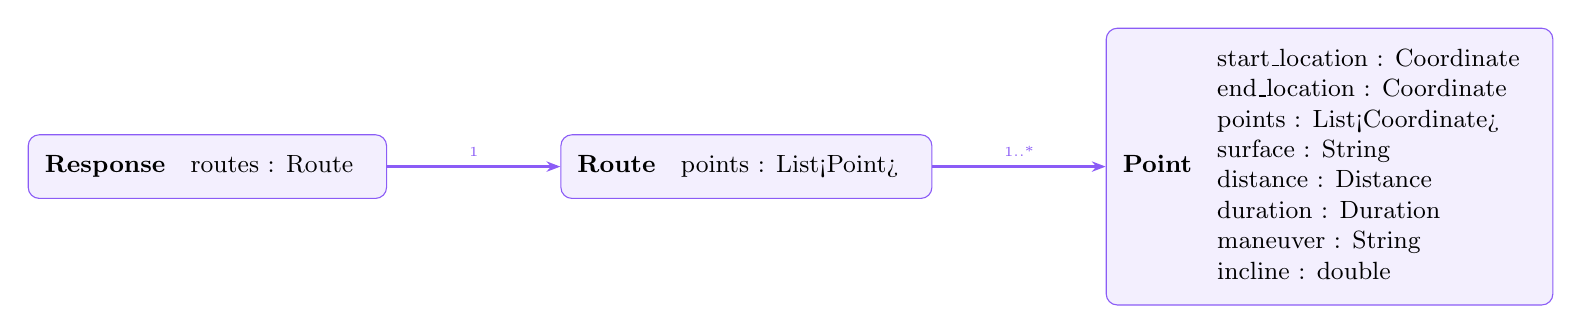
\begin{tikzpicture}[
  cls/.style={rectangle, draw=mypurple, fill=mypurple!10, rounded corners=4pt, minimum width=3.8cm, font=\small, inner sep=6pt},
  field/.style={font=\tiny\ttfamily, text=darkgray},
  arr/.style={-{Stealth[length=5pt]}, thick, color=mypurple},
  node distance=1.2cm and 2.0cm,
]
\node[cls] (resp) {
  \textbf{Response}\\[4pt]
  \begin{tabular}{l}
    \field{routes : Route}
  \end{tabular}
};
\node[cls, right=2.2cm of resp] (route) {
  \textbf{Route}\\[4pt]
  \begin{tabular}{l}
    \field{points : List<Point>}
  \end{tabular}
};
\node[cls, right=2.2cm of route] (point) {
  \textbf{Point}\\[4pt]
  \begin{tabular}{l}
    \field{start\_location : Coordinate}\\
    \field{end\_location : Coordinate}\\
    \field{points : List<Coordinate>}\\
    \field{surface : String}\\
    \field{distance : Distance}\\
    \field{duration : Duration}\\
    \field{maneuver : String}\\
    \field{incline : double}
  \end{tabular}
};

\draw[arr] (resp) -- (route) node[midway, above, font=\tiny] {1};
\draw[arr] (route) -- (point) node[midway, above, font=\tiny] {1..*};
\end{tikzpicture}
\caption{UML-style class diagram of the API response data model.}
\label{fig:datamodel}
\end{figure}

Each \texttt{Point} in the response represents one leg of the journey — a contiguous stretch of the route with a uniform surface type and a single dominant direction. The fields carry the following semantics:

\begin{description}[leftmargin=*, style=nextline]
  \item[\texttt{start\_location} / \texttt{end\_location}] Three-dimensional coordinates (latitude, longitude, elevation in metres) of the segment's start and end.
  \item[\texttt{points}] The full ordered list of 3D coordinates forming the segment's path. Clients use this to draw the route on a map.
  \item[\texttt{surface}] The OSM surface tag value for this segment (\textit{asphalt}, \textit{gravel}, \textit{grass}, \textit{unpaved}, etc.).
  \item[\texttt{distance}] A structured object containing the distance in feet (numeric) and a human-readable miles string.
  \item[\texttt{duration}] A structured object containing the estimated travel time in seconds (numeric) and a human-readable minutes string.
  \item[\texttt{maneuver}] The navigation instruction to execute at the \emph{end} of this segment (e.g., ``Turn left'', ``Go straight'', ``Reached'').
  \item[\texttt{incline}] The gradient of the segment expressed as a percentage. Positive values are uphill; negative values are downhill.
\end{description}

% ============================================================
\section{Automated Daily Map Updates}
\label{sec:mapupdate}

Keeping the routing map current is not a manual operation in MyPath. A scheduled background job runs every day at \textbf{1:23 AM} and performs a complete, zero-downtime refresh of the routing graph.

\subsection{Update Lifecycle}
\label{subsec:updatelifecycle}

The update proceeds through four sequential phases, as illustrated in Figure~\ref{fig:mapupdate}.

\begin{figure}[H]
\centering
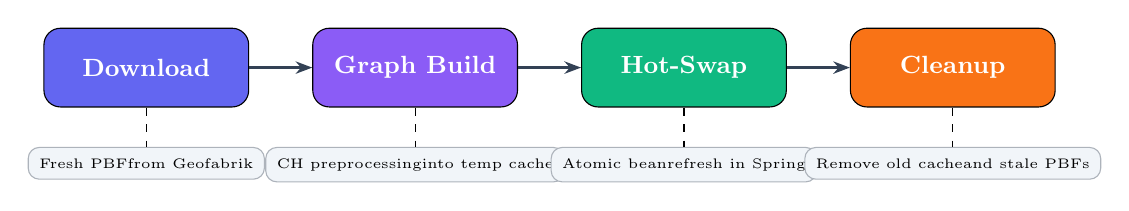
\begin{tikzpicture}[
  phase/.style={rectangle, rounded corners=6pt, draw, fill, text=white, minimum width=2.6cm, minimum height=1.0cm, font=\small\bfseries, text centered},
  detail/.style={rectangle, rounded corners=4pt, draw=darkgray!40, fill=lightgray, minimum width=2.6cm, font=\tiny, text centered, inner sep=4pt},
  arr/.style={-{Stealth[length=6pt]}, thick, color=darkgray},
  node distance=0.5cm and 0.6cm,
]
\node[phase, fill=myindigo] (p1) {Download};
\node[phase, fill=mypurple, right=0.8cm of p1] (p2) {Graph Build};
\node[phase, fill=mygreen, right=0.8cm of p2] (p3) {Hot-Swap};
\node[phase, fill=myorange, right=0.8cm of p3] (p4) {Cleanup};

\node[detail, below=of p1] (d1) {Fresh PBF\\from Geofabrik};
\node[detail, below=of p2] (d2) {CH preprocessing\\into temp cache};
\node[detail, below=of p3] (d3) {Atomic bean\\refresh in Spring};
\node[detail, below=of p4] (d4) {Remove old cache\\and stale PBFs};

\draw[arr] (p1) -- (p2);
\draw[arr] (p2) -- (p3);
\draw[arr] (p3) -- (p4);
\draw[dashed] (p1) -- (d1);
\draw[dashed] (p2) -- (d2);
\draw[dashed] (p3) -- (d3);
\draw[dashed] (p4) -- (d4);
\end{tikzpicture}
\caption{The four phases of the automated daily map update.}
\label{fig:mapupdate}
\end{figure}

\begin{enumerate}[leftmargin=*, label=\textbf{Phase \arabic{enumi}:}]
  \item \textbf{Download.} \texttt{MapService} downloads a fresh PBF file from the configured Geofabrik URL and saves it to the data store directory.
  \item \textbf{Graph Build.} \texttt{CustomGraphHopperConfig} constructs a new \texttt{GraphHopper} instance pointed at the fresh PBF and a temporary cache directory. The full CH preprocessing step runs, encoding the wheelchair profile across the updated road network.
  \item \textbf{Hot-Swap.} Once the new instance is fully initialised, it is atomically registered as the active \texttt{graphHopper} Spring bean using a \texttt{synchronized} swap. The old instance is then closed and its resources released. Because the swap is atomic, no routing request can observe a partially-initialised graph.
  \item \textbf{Cleanup.} The old routing graph cache directory is deleted. The temporary cache is moved into the primary cache path. Stale PBF files from previous update cycles are also deleted to reclaim disk space.
\end{enumerate}

\begin{greenbox}[Zero-Downtime Guarantee]
The server remains fully operational throughout all four phases. Incoming routing requests continue to be served by the old graph until the atomic swap completes in Phase 3, at which point they immediately begin using the new graph. There is no maintenance window and no restart required.
\end{greenbox}

\subsection{Data Freshness}
\label{subsec:freshness}

Geofabrik publishes updated regional extracts approximately every 24 hours, incorporating the latest contributions from the OpenStreetMap community worldwide. MyPath's daily update cycle therefore ensures that newly added pedestrian paths, changed surface classifications, updated smoothness assessments, and corrected slope data are reflected in routing results within one day of appearing in the OSM database.

% ============================================================
\section{Project Structure}
\label{sec:structure}

The MyPath source tree follows standard Spring Boot conventions, with packages named by their architectural role rather than by feature. Table~\ref{tab:structure} summarises the principal packages and their responsibilities.

\begin{table}[H]
\centering
\caption{Source package structure}
\label{tab:structure}
\begin{tabularx}{\textwidth}{@{}lX@{}}
\toprule
\textbf{Package} & \textbf{Responsibility} \\
\midrule
\texttt{configurations} & GraphHopper setup, CORS configuration, application wiring \\
\texttt{constants} & Shared named constants (file paths, URLs, slope thresholds, speed values) \\
\texttt{controller} & HTTP endpoint definitions; delegates immediately to services \\
\texttt{cron} & Scheduled map update job (\texttt{MapUpdateScheduler}) \\
\texttt{exceptions} & Custom domain exception types (\texttt{RouteNotFound}) \\
\texttt{exceptionHandler} & Global Spring exception handler; maps exceptions to HTTP responses \\
\texttt{filter} & Servlet filter for Bearer token authentication \\
\texttt{model} & Domain model classes (coordinates, segments, response objects, enums) \\
\texttt{service} & Business logic (routing, navigation, map download) \\
\texttt{utils} & Stateless utility functions (Haversine, bearing, incline, date, string) \\
\bottomrule
\end{tabularx}
\end{table}

The clean separation between \texttt{RoutingService} and \texttt{NavigationService} is a particularly important design choice. \texttt{RoutingService} knows only about GraphHopper; it is responsible for constructing the query and obtaining the raw response. \texttt{NavigationService} knows nothing about GraphHopper's internal representations; it operates exclusively on domain model objects. This boundary makes each service independently testable and makes future changes to the routing engine (for example, switching to a different graph backend) achievable without touching the navigation logic.

% ============================================================
\section{Deployment and Configuration}
\label{sec:deployment}

\subsection{Build Process}
\label{subsec:build}

MyPath is built using Gradle. The included \texttt{build\_script.sh} shell script invokes the Gradle \texttt{bootJar} task, which compiles the application and packages it as an executable JAR file at \texttt{build/libs/mypath-0.0.1-SNAPSHOT.jar}.

\subsection{Runtime Configuration}
\label{subsec:config}

The primary configuration file is \texttt{src/main/resources/application.properties}. The two most important settings are the application name and the API key used for Bearer token authentication. The API key should be set to a cryptographically random string of sufficient length before deployment and must never be committed to version control in production environments.

\subsection{Server Startup}
\label{subsec:startup}

The \texttt{start.sh} script launches the JAR in the background on port 8093, redirecting standard output and error to \texttt{mypath\_stdout.log}. On first startup (or when no routing graph cache exists), GraphHopper will download the configured PBF file if it is absent, build the full CH graph from scratch, and write the cache to disk. This initial build can take several minutes depending on the size of the regional extract; subsequent startups load the pre-built cache in seconds.

\subsection{Docker Support}
\label{subsec:docker}

A \texttt{Dockerfile} is included in the project root for containerised deployment. This allows MyPath to be deployed in any container orchestration environment (Docker Compose, Kubernetes, etc.) with consistent runtime behaviour regardless of the host operating system.

% ============================================================
\section{Summary}
\label{sec:summary}

MyPath addresses a genuine gap in the navigation technology landscape by delivering a routing engine that understands and respects the physical constraints of wheelchair travel. Its design reflects a principled combination of proven open-source components — GraphHopper, OpenStreetMap, and SRTM — held together by a clean Spring Boot service architecture.

The key design decisions that distinguish MyPath from a generic routing backend are:

\begin{itemize}[leftmargin=*]
  \item A \textbf{custom wheelchair routing profile} that enforces hard exclusions for inaccessible path types (steps, motorways, primary roads) and applies continuous gradient penalties.
  \item \textbf{Surface segmentation} of the returned route, enabling client applications to visualise and describe the terrain the user will traverse.
  \item \textbf{Turn-by-turn maneuver detection} derived from geodetic bearing mathematics rather than reliance on OSM turn restriction tags alone.
  \item \textbf{Per-segment incline reporting} computed from SRTM 3D elevation data, giving users and client applications awareness of gradients before they are encountered.
  \item \textbf{Zero-downtime daily map updates} via an atomic hot-swap of the GraphHopper instance, ensuring geographic accuracy without service interruption.
  \item \textbf{Contraction Hierarchies preprocessing} that delivers millisecond routing query times even over large geographic regions, making the engine suitable for real-time mobile navigation use cases.
\end{itemize}

Together these features form a routing backend that is not only functionally correct for wheelchair users but also operationally robust, well-structured, and straightforward to extend.

\end{document}
